\documentclass[a4paper,12pt,ngerman]{scrartcl}

% Language
\usepackage{polyglossia}
\setmainlanguage{german}

% Grafiken
\usepackage{graphicx}

% Make \today print in format "NN<st|nd|rd|th> MM YYYY"
\usepackage{isodate}
\origdate

\linespread{1.15}

% Titel anders formatieren mit: Command, Format, Label, Sep, Before-Code
\usepackage{titlesec}
\titleformat{\section}{\sffamily\Large\bfseries}{}{0pt}{}
\titleformat{\subsection}{\sffamily\large\bfseries}{}{0pt}{}

% Own pagestyle (header and footer)
\usepackage{fancyhdr}
\fancyhf{} % Clear header and footer content
\fancyhead[L]{{\small \textsf{WS 14/15, Informationsvisualisierung}}}
\fancyhead[C]{{\small \textsf{Übung 4}}}
\fancyhead[R]{{\small \textsf{\today}}}
\fancyfoot[C]{\thepage}

% Text in quotes
% Usage: \enquote{To be or not to be.}
\usepackage{csquotes}

% Subliminal refinements towards typographical perfection
\usepackage{microtype}

% Footnotes in section
\usepackage[stable]{footmisc}

% Better refs with \cref{}
\usepackage[capitalize,noabbrev]{cleveref}

% Borders
\usepackage[paper=a4paper,left=20mm,right=20mm,top=30mm,bottom=30mm]{geometry}

\usepackage{placeins}

\begin{document}
\pagestyle{fancy} % Activate own pagestyle

\section{Aufgabe 4.1 | Treemaps}
\subsection*{Slice-And-Dice}

Der Slice-And-Dice-Algorithmus schafft auf eine relativ einfache Art und Weise eine übersichtliche Treemap. Zunächst wird die Grundfläche entlang einer Achse in so viele Rechtecke geteilt, wie die Wurzel Kinder hat. Die Größe eines Rechtecks entspricht dabei immer der \enquote{Größe} des jeweiligen Kindes, die sich durch die Summe aller ihm untergeordneten Blätter errechnet (sofern es nicht selbst ein Blatt ist). Im nächsten Schritt werden dann die Kindeskinder nach dem gleichen Verfahren in der Fläche des entsprechenden Kindes verteilt, wobei die Partitionierung diesmal entlang der anderen Achse durchgeführt wird. So wird weiter verfahren bis alle Blätter erreicht sind (Breitensuche), wichtig ist dabei, dass in jedem Schritt die Achse gewechselt wird, nach der die Partitionierung stattfindet. Außerdem ist auch der Einsatz von Farben ein Muss, womit verschiedenste Attribute kodiert werden können. Das Ergebnis für den gegebenen Baum zeigt \cref{fig:sliceAndDice}.

\begin{figure}[ht]
    \centering
    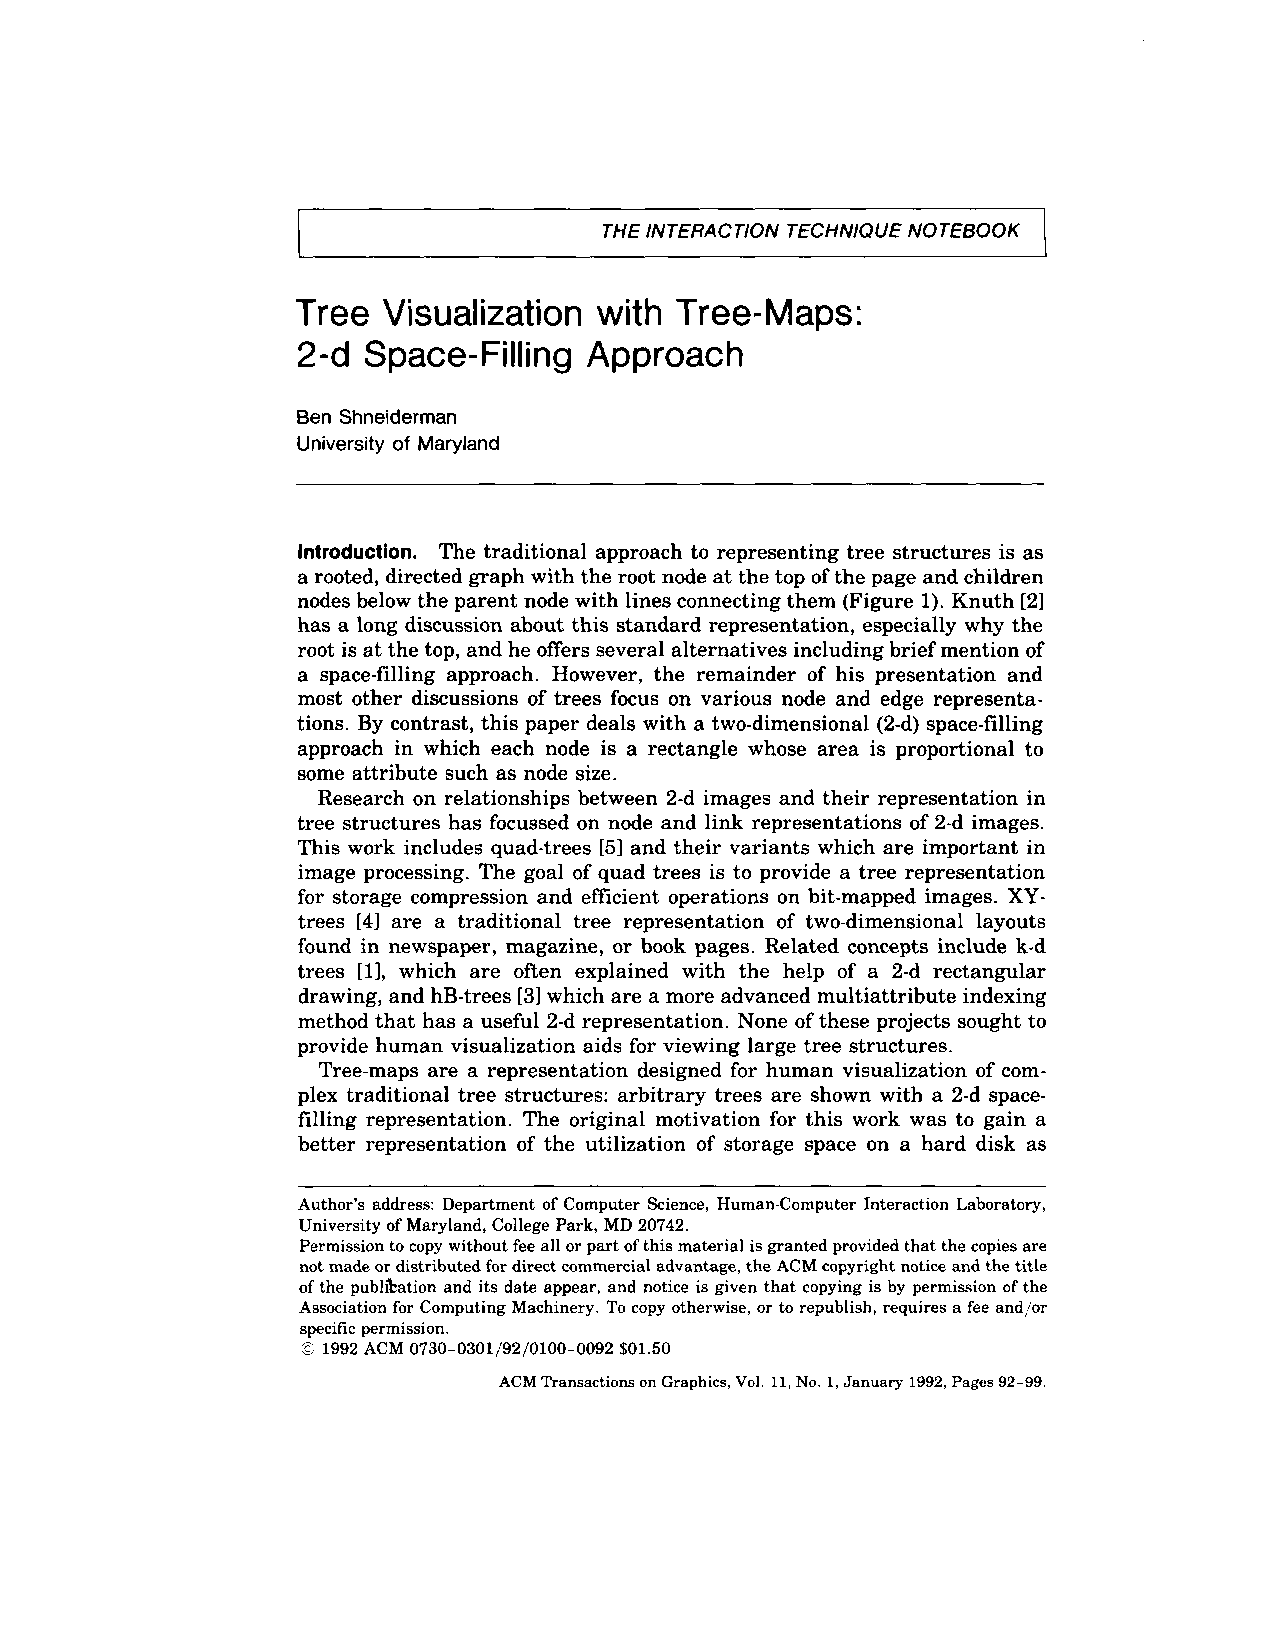
\includegraphics[height=10cm]{includes/SliceAndDice}
    \caption{Treemap - Slice-And-Dice-Algorithmus}
    \label{fig:sliceAndDice}
\end{figure}

\subsection*{Squarified Treemaps}

Eine Verbesserung zu den Treemaps stellen die Squarified Treemaps dar, wobei vermieden werden soll, dass lange, dünne Rechtecke entstehen, die für den Betrachter eher schwer zu vergleichen sind.

\begin{figure}[ht]
    \centering
    \includegraphics[height=10cm]{includes/SquarifiedTreemaps}
    \caption{Squarified Treemap}
    \label{fig:squarifiedTreemap}
\end{figure}

\begin{figure}[ht]
    \centering
    \includegraphics[height=10cm]{includes/SquarifiedTreemaps2}
    \caption{Squarified Treemap - absteigende Reihenfolge}
    \label{fig:squarifiedTreemap2}
\end{figure}
\FloatBarrier

Das Hauptziel dabei ist, das Seitenverhältnis der Rechtecke so nahe wie möglich an 1 zu bekommen. Der Algorithmus behandelt die Hierarchiestufen in einzelnen Schritten, ähnliche wie der zuvor beschriebene. Die Grundfläche wird an der jeweils längeren Seite zuerst geteilt und das erste Rechteck darin platziert. Danach wird überprüft, wie die Anordnung des zweiten Rechtecks erfolgen muss, um ein möglichst konstantes Seitenverhältnis zu erhalten. Diese Schritte werden für alle weiteren Elemente auf den jeweiligen Stufen der Hierarchie wiederholt. Um die Hierarchie visuell zu verdeutlichen, werden Rahmen eingesetzt.

In \cref{fig:squarifiedTreemap} ist eine Squarified Treemap zu gegebenem Baum zu finden. Da bei diesem Algorithmus eine absteigende Reihenfolge meist bessere Ergebnisse bringt, wurden die Elemente des gegebenen Baumes also sortiert und nochmals eine Squarified Treemap erzeugt (siehe \cref{fig:squarifiedTreemap2}. Weit unterscheiden sich die beiden Treemaps in diesem Fall nicht, nur in dem 10er-Bereich mit den Einzelwerten 3, 2, 2, 2 und 1 ist eine bessere Aufteilung entstanden.

\subsection*{Vergleich}

Der große Vorteil der mit dem Slice-And-Dice-Algorithmus erzeugten Treemap ist, dass die Hierarchie gut sichtbar bleibt. Durch die abwechselnd horizontale und vertikale Ausrichtung der Rechtecke bekommt man relativ schnell das Gefühl dafür, auf welcher Stufe ein einzelnes Rechteck angeordnet ist.

Der Nachteil dieser Methode ist jedoch, dass die Rechtecke oft sehr lang und dünn werden. Dadurch ist ihre Fläche für den Menschen relativ schwer einschätzbar und Vergleiche zu anderen Rechtecken sind kaum zu ziehen.

Dem begegnen die Squarified Treemaps und versuchen möglichst quadratische Rechtecke  zu verwenden. Dies erleichtert das Verständnis und zudem die visuelle Darstellung. Die Rechtecksbegrenzungen nehmen durch die fast quadratische Aufteilung weniger Platz in Anspruch und die Rechtecke sind bei einer interaktiven Grafik leichter anzuklicken.

Da jedoch die Hierarchie zunächst schwer erkennbar ist, müssen verschieden breite Rahmen o. Ä. eingesetzt werden, wodurch wieder mehr Platz verbraucht wird.

Einen klaren Favoriten sehe ich hier also nicht, es kommt immer darauf an, welche Informationen gerade von Bedeutung sind und wie gut Farben, Rahmen, Schattierungen usw. eingesetzt werden.

\newpage

\section{Aufgabe 4.2 | DNS-Vergleich mit Dendroscope}
\subsection*{Vergleich mittels Galled Network}

In \cref{fig:galledNetwork} ist ein \enquote{galled network}, eine Verallgemeinerung eines \enquote{galled trees}, zu sehen. Der Algorithmus versucht hier beide Bäume auf Blattebene zu verbinden. Anschließend werden die beiden vorher separaten Bäume in einem Netzwerk (mit einer einem Baum möglichst ähnlichen Darstellelung) dargestellt. Der schwarze Anteil gehört zum ersten Baum, der blaue Anteil ist anschließend zum diesem hinzugefügt worden sodass ein Vergleich möglich ist.

\begin{figure}[ht]
    \centering
    \includegraphics[width=\textwidth]{includes/GalledNetwork}
    \caption{Galled Network}
    \label{fig:galledNetwork}
\end{figure}

\subsection*{Vergleich mittels Tanglegram}

Das Tanglegram stellt beide Bäume nebeneinander dar und verbindet anschließend die gleichen Kategorien (auch: Taxa) mit grauen horizontalen Linien.

\begin{figure}[ht]
    \centering
    \includegraphics[height=23cm]{includes/Tanglegram}
    \caption{Tanglegram}
    \label{fig:tanglegram}
\end{figure}

Bei beiden Darstellungen mussten keine weiteren Eingabeparameter verwendet werden.

\end{document}
